\chapter{Evaluation}
In der Evaluation werden drei Aspekte betrachtet: Klassifizierungsgenauigkeit, Robustheit und Resourcennutzung.
Bei der Klassifizierungsgenauigkeit wird einerseits die Standorterkennung und andererseits die Anomalieerkennung evaluiert.
Dabei wird sowohl auf verschiedene Größen von FFNN und Entscheidungswälder eingegangen,
als auch auf verschieden viele zu unterscheidenden Standorte.
\newline
\newline
Bei der Robustheit wird auf den Fehler des besten FFNN und Entscheidungswald bei verschiedene Fehlerszenarien eingegangen.
Diese bestehen aus fehlerhafte Sensordaten durch Rauschen oder ausgefallenen Sensoren,
Routen mit permutierten Teilstücken und Routen, bei denen simuliert wird, dass der letzte Standort übersprungen wurde.
\newline
\newline
Bei der Resourcennutzung wird auf die Programmgröße und die Ausführungszeit der besten ML-Modelle eingegangen.
Außderdem wird der Energieverbrauch für verschiedene Szenarien eingeschätzt.

\section{Metriken}
In dieser Arbeit werden verschiedene Metriken zur Ermittlung der Klassifizierungsgenauigkeit ermittelt.
Zunächst die übliche Klassifizierungsgenauigkeit (\ref{formular:simple_accuracy}), in der die Anzahl der korrekt klassifizierten Standorte mit der Gesamtanzahl verglichen werden.
\begin{align}
    \label{formular:simple_accuracy}
    P(A) := \frac{\text{Anzahl korrekter Klassifizierungen}}{\text{Gesamtanzahl}}
\end{align}
Die zweite Metrik (\ref{formular:accuracy_metrik2}) betrachtet die Klassifizierungsgenauigkeit unter Tolerierung, dass ein Standort
fünf bzw. zehn Klassifizierungen kontinuierlich zu früh oder zu spät verlassen wurde,
d.~h. Fehlklassifizierungen werden vernachlässigt, wenn kontinuierlich der letzte korrekte Standort bzw. der nächste korrekte
Standort klassifiziert wird mit einer Gesamttoleranz von fünf bzw. zehn Klassifizierungen.
\begin{flalign}
    \label{formular:accuracy_metrik2}
    &\epsilon \in \{5, 10\} \nonumber\\
    &L := \text{Menge von dem ML-Modell klassifizierten Standorte.} \nonumber\\
    &K := \text{Menge von den wirklichen Standorten.} \nonumber\\
    &\Phi(i) := \text{Index von dem nächsten Standort.} \nonumber\\
    &\Psi(i) := \text{Index von dem vorherigen Standort.} \nonumber\\
    &\Omega(i) := \Phi(i)-i\leq\epsilon\wedge\hspace{-0.3cm} \bigwedge\limits_{i\leq q \leq \min(\#K, \Phi(i))}\hspace{-0.3cm} L_q=K_{\Phi(i)} \nonumber\\
    &\Theta(i) := i-\Psi(i)\leq\epsilon\wedge\hspace{-0.3cm} \bigwedge\limits_{\max(0, \Psi(i))\leq q \leq i}\hspace{-0.3cm} L_q=K_{\Psi(i)} \nonumber\\
    &P(B) := \frac{\#\{L_i | L_i=K_i \vee \Omega(i) \vee \Theta(i)\text{ für } i\in\{0, 1, ..., \#L - 1\}\}}{\#K}
\end{flalign}
Zuletzt zwei Metriken bei denen die Klassifizierungsgenauigkeit bestimmt wird, unter der Bedingung, dass der vorherige
Standort korrekt (\ref{formular:accuracy_previous_was_correct}) bzw. falsch (\ref{formular:accuracy_previous_was_wrong}) war.
\begin{align}
    \label{formular:accuracy_previous_was_correct}
    P(C) := \frac{\text{Anzahl korrekter Klassifizierungen, wenn vorheriger Standort korrekt war}}{\text{Alle Klassifizierungen, wenn vorheriger Standort korrekt war}}
\end{align}
\begin{align}
    \label{formular:accuracy_previous_was_wrong}
    P(D) := \frac{\text{Anzahl korrekter Klassifizierungen, wenn vorheriger Standort falsch war}}{\text{Alle Klassifizierungen, wenn vorheriger Standort falsch war}}
\end{align}
\section{Klassifizierungsgenauigkeit der Standorte}
Die Klassifizierungsgenauigkeit der ML-Modelle zur Standorterkennung wurde mit verschiedenen Konfigurationen über komplexer werdende Datenmengen evaluiert.
In Kapitel \ref{sec:model_dt} und Kapitel \ref{sec:model_ffnn} werden die einzelnen Konfigurationen der ML-Modelle beschrieben.
Die Komplexität wird über die Anzahl der Standorte definiert.
Um die Anzahl der Standorte zu erhöhen, wurden die Datenmengen um weitere Routen erweitert.
Dies impliziert aber, dass die Testmengen nicht vergleichbar sind unter den Standortanzahlen, da mit jeder Route auch die Testmenge erweitert wird.
Die berechneten Klassifizierungswahrscheinlichkeiten sind jeweils der Durchschnitt der Klassifizierungswahrscheinlichkeiten aller Routen in der Testmenge.
\newline
\newline
Außerdem unterscheiden sich die Enkodierungsansätze je nach Standortanzahl.
Für die Standortanzahlen 9, 17, 25 und 52 wurde der Enkodierungsansatz verwendet, bei denen nur die Knoten und ein zusätzlicher unbekannter Standort betrachtet wird.
Für die Standortanzahlen 16, 32, 48 und 102 wurde der Enkodierungsansatz verwendet, bei denen Knoten und Kanten betrachtet werden.
Ein besserer Ansatz, um Daten mit beliebiger Komplexität zu generieren wird in Kapitel \ref{chapter:discussion} diskutiert.
\newline
\newline
Zunächst wird die Klassifizierungsgenauigkeit $P(A)$ im Vergleich zu Mians Ergebnissen betrachtet.
Mian konnte mit einem WFFNN bei einer Route mit drei Pfaden und 14 Standorten eine Klassifizierungsgenauigkeit von 94,1\% erreichen \cite{naveedThesis}.
Abbildung \ref{fig:best_dt_acc_vs_knn_acc_vs_cont} vergleicht die Klassifizierungsgenauigkeiten der
Entscheidungsbaum basierten Klassifizierer und FFNN über verschiedene Standortkomplexitäten.
Dabei wurde stets die höchste Klassifizierungsgenauigkeiten aller evaluierten Konfigurationen ausgewählt.
Gezeigt werden sowohl die Klassifizierungsgenauigkeiten auf die Testmengen die korrekt beschriftet sind und die, die von den ML-Modellen beschriftet sind.
\begin{figure}[h!]
    \centering
    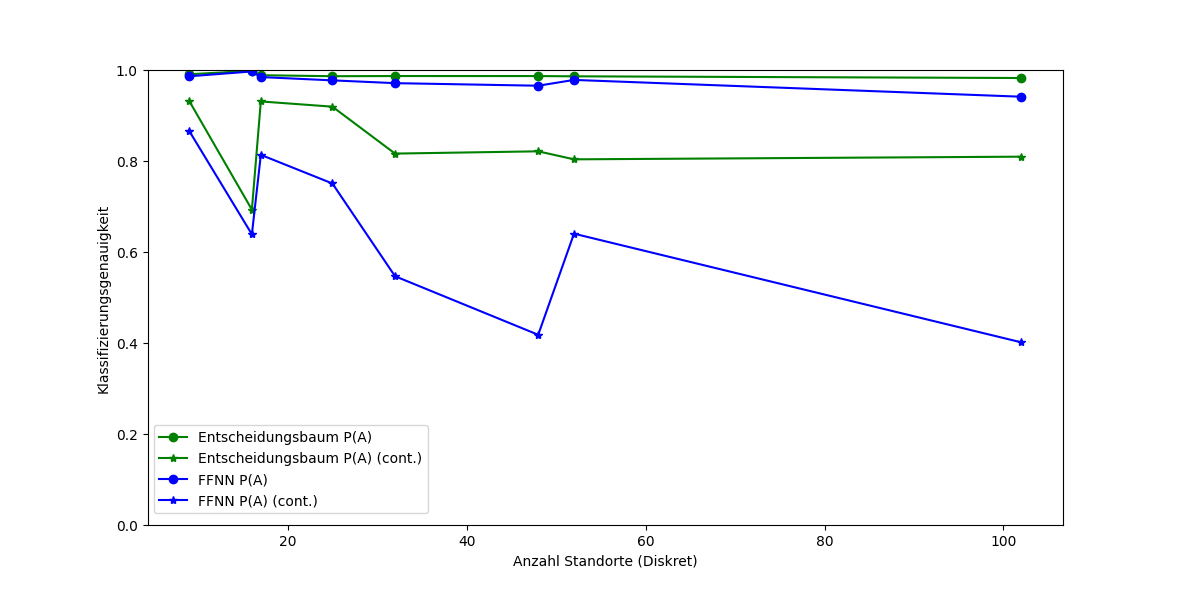
\includegraphics[width=\linewidth]{images/best_dt_vs_knn_acc_vs_acc_cont.png}
    \caption{Die besten Klassifizierungsgenauigkeiten aller evaluierten Konfigurationen der ML-Modelle über alle Standortkomplexitäten.}
    \label{fig:best_dt_acc_vs_knn_acc_vs_cont}
\end{figure}
\newline
\newline
Mian hat in seiner Evaluation die Klassifizierungsgenauigkeit $P(A)$ betrachtet.
Die in dieser Arbeit evaluierten Standortkomplexität, die Mians Evaluation am nächsten kommt ist 16.
Im Vergleich ist der beste Entscheidungsbaum basierte Klassifizierer mit einer Klassifizierungsgenauigkeit von 99,9\%, 5,8 Prozentpunkte besser
und das beste FFNN mit einer Klassifizierungsgenauigkeit von 99,79\%, 5,69 Prozentpunkte besser (Tabelle \ref{tab:predictions_by_acc}).
\newline
\newline
Dies betrachtet aber nicht den propagierten Fehler, der durch die Rekursion der ML-Modelle entsteht.
In Abbildung \ref{fig:best_dt_acc_vs_knn_acc_vs_cont} ist zu sehen, dass die Klassifizierungsgenauigkeit signifikant geringer ist bei allen Standortkomplexitäten.
Besonders mit der Standortkomplexität 16 ist die Klassifizierungsgenauigkeit signifikant geringer, wobei dies eine Artefakt der Enkodierungsmethode sein kann,
da bei der Standortkomplexität 17 immernoch Entscheidungsbaum basierte Klassifizierer mit einer Klassifizierungsgenauigkeit von 95,86\% gefunden wurden (Tabelle \ref{tab:predictions_by_acc_cont}).
Die FFNNS hingegen erreichen lediglich maximal 88,1\% bei dieser Standortkomplexität.
\newline
\newline
Aus Tabelle \ref{tab:predictions_by_acc_10_cont} können die Klassifizierungsgenauigkeiten $P(B=10)$ entnommen werden.
Der Entscheidungsbaum basierte Klassifizierer skaliert dabei sehr gut mit der steigenden Standortkomplexität.
Aber einer Standortkomplexität von 32 wird konnte aber nurnoch eine Klassifizierungsgenauigkeit von 91,35\% erreicht werden, die bis auf 87,87\% bei 102 Standorten fällt.
Als beste maximale Baumhöhe hat sich 16 herausgestellt, wobei 32 und 64 marginal schlechtere Ergebnisse produzierten.
Eine maximale Baumhöhe von 8 war nicht ausreichend und hat sich hat deutlich schlechtere Ergebnisse erzielt.
Bei gleicher Waldgröße haben die maximalen Baumhöhen und 32 und 64 equivalente Ergebnisse produziert.
Die verschiedenen Waldgrößen unterscheiden sich nicht stark.
Eine Waldgröße von 8 hat nur marginal schlechtere Ergenisse bei 102 Standorten erzielt, als die Waldgrößen 16, 32 und 64.
Aus diesem Grund ist eine Waldgröße von 8 ausreichend, oder könnte womöglich immernoch reduziert werden.
\newline
\newline
Die evaluierten FFNNs skalieren deutlich schlechter als die Entscheidungsbaum basierten Klassifizierer mit steigender Standortkomplexität.
Besonders die FFNNs der Standortkomplexitäten, die das Enkodierungsverfahren der Kanten und Knoten nutzte,
konnten signifikant schlechtere Klassifizierungsergebnisse erzielen als die FFNNs die das andere Enkodierungsverfahren nutzten.
Aus den Daten ist nicht zu schließen, wie sich die Anzahl der Schichten und Neuronen pro Schicht auf die Klassifizierungsgenauigkeit auswirkt.
Für geringe Standortkomplexitäten haben vermehrt kleine FFNNs besser abgeschnitten und für große Standortkomplexitäten vermehrt große FFNNs.
\begin{table}[h!]
    \hspace{-1.5cm}
    \begin{tabular}{ | c | c | c | c | c | c | c | c | c | c | }
        \hline
        \multicolumn{2}{ | l |}{$P(B=10)_{\text{cont}}$ über Standorte} & 9 & 16 & 17 & 25 & 32 & 48 & 52 & 102 \\\hline
        \multicolumn{10}{| l |}{\textbf{Entscheidungswälder}}\\\hline
        Waldgröße & Max. Baumgröße & \multicolumn{8}{ c |}{}\\\hline
        16 & 8 & 99.88 & 81.69\% & 99.50\% & 94.21\% & 82.88\% & 88.40\% & 85.72\% & 79.01\% \\\hline
        16 & 16 & 99.78 & 77.30\% & 99.73\% & 93.40\% & 91.35\% & 92.86\% & 89.86\% & 89.10\% \\\hline
        16 & 32 & 99.78 & 77.00\% & 99.83\% & 98.31\% & 86.55\% & 92.60\% & 90.66\% & 85.69\% \\\hline
        16 & 64 & 99.78 & 77.00\% & 99.83\% & 98.31\% & 86.55\% & 92.60\% & 90.66\% & 85.69\% \\\hline
        8 & 32 & 98.92 & 92.79\% & 99.66\% & 98.10\% & 90.27\% & 91.45\% & 89.46\% & 85.11\% \\\hline
        16 & 32 & 99.78 & 77.00\% & 99.83\% & 98.31\% & 86.55\% & 92.60\% & 90.66\% & 85.69\% \\\hline
        32 & 32 & 99.79 & 78.06\% & 99.63\% & 97.52\% & 88.83\% & 93.33\% & 89.20\% & 86.92\% \\\hline
        64 & 32 & 99.69 & 84.66\% & 99.82\% & 97.62\% & 89.65\% & 93.31\% & 86.15\% & 87.87\% \\\hline
        32 & 64 & 99.79 & 78.06\% & 99.63\% & 97.52\% & 88.83\% & 93.33\% & 89.20\% & 86.92\% \\\hline
        \multicolumn{10}{| l |}{\textbf{Feed Forward neuronale Netzwerke}}\\\hline
        \#Schichten & \#Neuronen & \multicolumn{8}{ c |}{}\\\hline
        1 & 16 & 99.65 & 76.69\% & 93.25\% & 83.76\% & 45.93\% & 65.16\% & 76.85\% & 42.39\% \\\hline
        1 & 32 & 99.77 & 77.04\% & 93.47\% & 84.28\% & 63.63\% & 64.21\% & 76.40\% & 44.73\% \\\hline
        1 & 64 & 99.69 & 68.52\% & 95.35\% & 88.93\% & 50.44\% & 83.60\% & 80.52\% & 33.87\% \\\hline
        1 & 128 & 99.10 & 75.39\% & 92.96\% & 91.02\% & 52.27\% & 55.62\% & 82.18\% & 42.56\% \\\hline
        2 & 32 & 98.59 & 63.99\% & 96.98\% & 87.72\% & 68.52\% & 73.21\% & 79.07\% & 35.48\% \\\hline
        4 & 32 & 99.61 & 71.53\% & 93.63\% & 93.19\% & 49.47\% & 52.64\% & 82.16\% & 38.66\% \\\hline
        8 & 32 & 92.74 & 62.31\% & 86.52\% & 86.57\% & 36.36\% & 71.92\% & 75.98\% & 51.15\% \\\hline
        4 & 64 & 99.06 & 67.74\% & 93.76\% & 94.15\% & 54.47\% & 47.75\% & 82.08\% & 47.55\% \\\hline
    \end{tabular}
    \caption{Metrik $P(B=10)_{\text{cont}}$ über Standorte und verschiedenen Konfigurationen der ML-Modelle.}
    \label{tab:predictions_by_acc_10_cont}
\end{table}
\section{Klassifizierungsgenauigkeit der Anomalien}
\label{sec:eval_anomalieerkennung}
Bei der Anomalieerkennung werden Entscheidungswälder und FFNNs mit den besten ML-Modellen zur Standorterkennung trainiert und mit den drei Baseline-Modellen verglichen.
Tabelle \ref{tab:anomaly_detection_prediction_accuracy} zeigt die Klassifizierungsgenauigkeiten über die verschiedenen Standortkomplexitäten,
wobei die Klassifizierungsgenauigkeit $P(A)$ nochmal genauer aufgeschlüsselt ist in den Anteil der korrekten Klassifizierungen, wenn eine bzw. keine Anomalie vorlag.
Die trainierten FFNNs geben stets aus, dass keine Anomalie vorliegt.
Es ist unklar, warum die FFNNs sich so verhalten.
\begin{table}[h!]
    \hspace{-1cm}
    \begin{tabular}{ | l | c | c | c | c | c | c | c | c | }
        \hline
        Standorte & 9 & 16 & 17 & 25 & 32 & 48 & 52 & 102 \\\hline
        \multicolumn{9}{ | l |}{$P(A)$}\\\hline
        Entscheidungswald & 82,59\% & 81,19\% & 87,14\% & 84,91\% & 79,06\% & 83,47\% & 81,93\% & 76,00\% \\\hline
        FFNN & 77,88\% & 77,88\% & 77,88\% & 77,88\% & 77,88\% & 77,88\% & 77,88\% & 77,88\% \\\hline
        Topologie (DT) & 84,77\% & 30,57\% & 83,51\% & 79,76\% & 28,63\% & 24,97\% & 80,55\% & 29,47\% \\\hline
        Topologie (KNN) & 86,10\% & 52,17\% & 77,72\% & 79,30\% & 45,06\% & 41,92\% & 74,77\% & 43,55\% \\\hline
        \multicolumn{9}{ | l |}{Anteil korrekt klassifiziert, indem Anomalie vorlag}\\\hline
        Entscheidungswald & 34,86\% & 35,52\% & 52,58\% & 50,92\% & 32,21\% & 50,64\% & 23,21\% & 1,92\% \\\hline
        FFNN & 0,00\% & 0,00\% & 0,00\% & 0,00\% & 0,00\% & 0,00\% & 0,00\% & 0,00\% \\\hline
        \multicolumn{9}{ | l |}{Anteil korrekt klassifiziert, indem keine Anomalie vorlag}\\\hline
        Entscheidungswald & 96,14\% & 94,41\% & 97,05\% & 95,83\% & 92,48\% & 93,13\% & 98,96\% & 97,18\% \\\hline
        FFNN & 100,00\% & 100,00\% & 100,00\% & 100,00\% & 100,00\% & 100,00\% & 100,00\% & 100,00\% \\\hline
    \end{tabular}
    \caption{$P(A)$ über Standorte und Modelle zur Anomalieerkennung.}
    \label{tab:anomaly_detection_prediction_accuracy}
\end{table}
\newpage
Die Entscheidungswälder hingegen eignen sich besser für den Anomalieerkennungszweck.
Es werden zwischen 1,92\% und 52,58\% der Anomalien erkannt und zwischen 1,04\% und 7,52\% falsch als Anomalien erkannt.
Die Klassifizierungsgenauigkeit des Entscheidungswaldes zur Anomalieerkennung ist abhängig von der Klassifizierungsgenauigkeit zur Standorterkennung
und von der Standortkomplexität.
Je besser das Standorterkennungsmodell und je höher die Standortkomplexität, desto höher ist die Anomalieerkennungsrate.
Aus diesem Grund ist die Klassifizierungsgenauigkeit bei den Standortkomplexitäten, die mit der Kodierungsmethode mit Kanten und Knoten zusammenhängen,
geringer, als bei der Kodierungsmethode, bei der nur die Knoten kodiert werden.
\newline
\newline
Abbildung \ref{fig:true_vs_predicted_anomaly} zeigt einen Auscchnitt der Anomalietestmenge, worauf der Entscheidungswald der Standortkomplexität 17 angewendet wurde.
Die Anomalie wird nicht kontinuierlich erkannt und es werden auch fälschlicherweise Standorte als Anomalien klassifiziert.
Allerdings treten falsch-positive Ergebnisse nur vereinzelt auf, wohingegen bei einer Anomalie, sehr häufig eine Anomalie erkannt wird.
Die falsch-positiven Ergebnisse können somit durch Ausnutzen dieser Fluktuationen vermieden werden,
indem beispielweise ein Schwellenwert an Ausschlägen in einer bestimmten Zeit eingeführt wird.
\begin{figure}[h!]
    \centering
    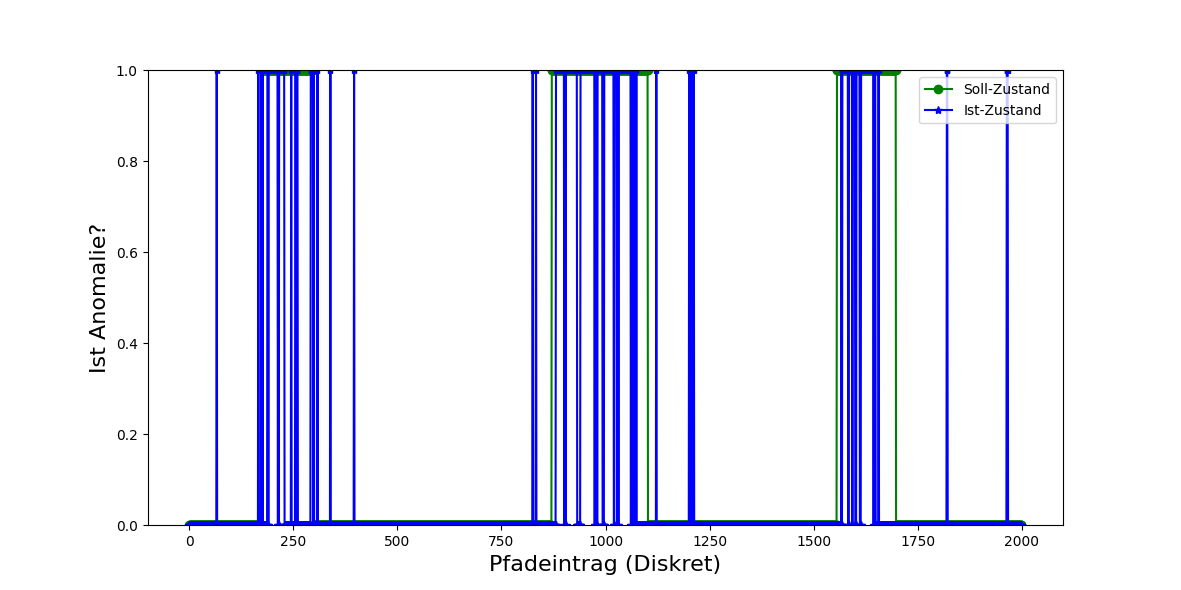
\includegraphics[width=\linewidth]{images/anomaly_true_vs_predicted.png}
    \caption{Ausschnitt der Klassifizierungsergebnisse auf der Anomalietestmenge mit dem Entscheidungswald der Standortkomplexität 17. }
    \label{fig:true_vs_predicted_anomaly}
\end{figure}

\section{Signifikanz der Features}
\begin{itemize}
    \item Signifikanz der Features
    \item Einfluss von einzelnen Features für die Klassifizierungsgenauigkeit(?) => Last Distinct location möglicherweise schlecht, da die eigentliche Last Distinct Location oft durch fehlende Interrupts übersprungen wird
    \item Welche Feature werden genutzt? => Abhängig von Feature Importance und wie günstig zu berechnen
    \item Ist es sinnvoll für jeden Ort ein Feature zu haben, dass auf eins gesetzt wird, wenn der Ort erkannt wurde und ansonsten exponentiell abfällt. Wie schnell sollte es fallen, wenn ja?
\end{itemize}

\section{Benötigte Anzahl der Trainingsdaten}
\begin{itemize}
    \item Werden mehr Trainingsdaten benötigt mit steigender Ort Anzahl? Wenn ja wie viel? (Hier oder bei ML-Modell Training)
    \item Wie viele Trainingsdaten werden benötigt?
    \begin{itemize}
        \item Um KNN zu trainieren?
        \item Um Entscheidungsbaum zu trainieren?
        \item Ggf. Unterschiede klären
        \item (Gehört das schon in eine Evaluation, oder ist das hier okay?)
    \end{itemize}
\end{itemize}

\section{Fehlertoleranz}
Bei der Fehlertoleranz wird die Fähigkeit der ML-Modelle untersucht, trotz fehlerhafter Sensordaten Standorte zu erkennen.
Dafür wurden für jeden Sensor modifizierte Testmengen erstellt.
Die erste Testmenge fügt ein Rauschen von 5\% hinzu und die zweite Testmenge simuliert den Ausfall des Sensors, indem alle Sensorwerte genullt werden.
Zudem wurde untersucht, was passiert wenn die Sensorenbox nicht dem trainierten Pfad folgt, indem die Testmenge permutiert wurde.
Damit Entscheidungswald und FFNN fair verglichen werden können, werden die besten ML-Modelle der Standortkomplexität 9 verwendet.
\newline
\newline
Tabelle \ref{tab:robustness} zeigt die Differenz der Klassifizierungsgenauigkeiten $P(A)_{\text{cont}}$ und $P(A)$ von den modifizierten Testmengen zur originalen Testmenge.
Die Testmengen mit einem Rauschen von 5\% wurde ausgelassen, da es keine Auswirkung auf die Klassifizierungsgenauigkeit hatte.
Vermutlich ist 5\% Rauschen zu wenig, um einen Einfluss auszuüben.
\begin{table}[h!]
    \hspace{-1.25cm}
    \begin{tabular}{ | l | c | c | c | c | }
        \hline
        Testmenge & Entscheidungswald & FFNN & Entscheidungswald & FNNN \\\hline
        & \multicolumn{2}{ c }{mit Rückwärtskante} & \multicolumn{2}{| c |}{ohne Rückwärtskante} \\\hline
        Licht & 4.46\%-Pkt. & 4.65\%-Pkt. & 5.28\%-Pkt. & 6.93\%-Pkt \\\hline
        Geräusch & 3.20\%-Pkt. & 5.00\%-Pkt. & 1.63\%-Pkt. & 5.11\%-Pkt. \\\hline
        Temperatur & 15.15\%-Pkt. & 6.60\%-Pkt. & 8.10\%-Pkt. & 13.50\%-Pkt. \\\hline
        Ausrichtung zum Magnetfeld & 3.32\%-Pkt. & 19.94\%-Pkt. & 2.51\%-Pkt. & 2.78\%-Pkt. \\\hline
        WLAN-Zugangspunkte & 2.60\%-Pkt. & 22.65\%-Pkt. & 3.74\%-Pkt. & 14.13\%-Pkt. \\\hline
        Accelerometer & 1.41\%-Pkt. & 9.52\%-Pkt. & 0.62\%-Pkt. & 1.33\%-Pkt. \\\hline
        Gyroskop & 8.52\%-Pkt. & 4.58\%-Pkt. & 0.91\%-Pkt. & 3.30\%-Pkt. \\\hline
        Permutierte Testmenge & 2.27\%-Pkt. & -0.13\%-Pkt. & 0.47\%-Pkt. & 0.93\%-Pkt. \\\hline
        \textbf{Durchschnitt} & \textbf{5,8\%-Pkt.} & \textbf{9,1\%-Pkt.} & \textbf{2,91\%-Pkt.} & \textbf{6,00\%-Pkt.} \\\hline
    \end{tabular}
    \caption{Fehler der modifizierten Testmengen zur originalen Testmenge.}
    \label{tab:robustness}
\end{table}
\newline
\newline
Die ML-Modelle mit und ohne Rückwärtskante sind robust gegenüber der Nullung der Features und gegenüber der permutierten Testmenge.
Aus der Menge stechen die Fehler durch die Nullung der Features des Temperatur- und Magnetfeldsensors sowie der WLAN-Zugangspunkte heraus.
Außerdem ist der Fehler durch die Nullung der Features des Accelerometers und Gyroskops bei den ML-Modellen mit Rückwärtskanten
deutlich größer als bei den ML-Modellen ohne Rückwärtskante.
\newline
\newline
Die Permutationswichtigkeit hat den Features des Temperatursensors eine geringere Wichtigkeit zugeordnet, als die Nullung es tut.
Dies ist dadurch begründet, dass die Sensordaten des Temperatursensors mit wenigen Ausnahmen sehr homogen sind.
Für den Temperatursensor wird eine Umgebungstemperatur simuliert, die sich nur verändert, wenn die Sensorenbox einer Wärmequelle näher kommt.
Für den größten Teil der Daten misst der Temperatursensor die Umgebungstemperatur, weswegen eine permutation keinen großen Fehler verursacht.
Die Nullung dieser Sensordaten hingegen deutet auf eine Wärmequelle hin, die die Umgebungstemperatur verringert.
Dieses Ereignis ist im Vergleich zu einer Erhöhung der Umgebungstemperatur selten, weswegen die Nullung einen großen Fehler verursacht.
Würde dieses Ereignis häufiger vorkommen, wäre der Fehler vermutlich geringer.
\newline
\newline
Das FFNN mit Rückwärtskante hat im Vergleich zu den anderen ML-Modellen einen deutlich größeren Fehler, wenn die Features des Magnetfeldsensors genullt werden.
Diese Anomalie ist entgegen den Erwartungen der Permutationswichtigkeit, insbesondere da die anderen ML-Modelle
höhere Permutationswichtigkeiten für die Features des Magnetfeldsensors erzeugt haben.
Es ist unklar, warum das FFNN, im Vergleich zu den anderen ML-Modellen, dem so anfällig ist.
\newline
\newline
Die FFNNs erzeugen einen großen Fehler, wenn die WLAN-Zugangspunkte genullt werden.
Dies stimmt mit den Ergebnissen der Permutationswichtigkeit überein.
Insgesamt bilden die Features der WLAN-Zugangspunkte 14,7\% aller Features, wobei die Werte bei der Eingabeschicht binär sind.
Vermutlich ist aus diesem Grund der Einfluss dieser Features beim FFNN im Vergleich zu den Entscheidungswäldern so groß.
\newline
\newline
Die Permutation der Testmenge hat nur einen geringen Fehler verursacht.
Dies war bei allen ML-Modellen zu erwarten, da das interne Datenfenster mit drei Einträgen sehr klein ist
und die Features der vorherigen Standorte bereits nach wenigen Klassifizierungen korrigiert werden.
Dementsprechend ist der Fehler bei den ML-Modellen ohne Rückwärtskante auch deutlich kleiner als bei den ML-Modellen mit Rückwärtskante.
\newpage
Im Durchschnitt sind die ML-Modelle ohne Rückwärtskante robuster als die ML-Modelle mit Rückwärtskante.
Die Entscheidungswälder sind robuster als die FFNNs.
Der beobachtete Fehler korreliert aber mit der Klassifizierungsgenauigkeit der ML-Modelle (Abbildung \ref{fig:best_dt_vs_knn_fb_vs_no_fb}).
Der Entscheidungswald mit Rückwärtskante, der marginal bessere Klassifizierungsgenauigkeiten erzielt hat, als das FFNN ohne Rückwärtskante,
hat einen marginal geringeren Fehler im Test erzielt.
\newline
\newline
Tabellen \ref{tab:predictions_by_acc_pic_cont} und \ref{tab:predictions_by_acc_pic_wo_fb} geben die Klassifizierungsgenauigkeit $P(C)_{\text{cont}}$ bzw. $P(C)$ an.
Diese geben die Wahrscheinlichkeit an, dass ein Standort korrekt klassifiziert wird, wenn der Standort zuvor falsch klassifiziert wurde.
Wie zu erwarten ist die Wahrscheinlichkeit bei den ML-Modellen ohne Rückwärtskante deutlich größer.
Bei einer Standortkomplexität von 9 Orten benötigt ein Entscheidungswald mit Rückwärtskante ca. 5,3 Klassifizierungen,
ein FFNN mit Rückwärtskante ca. 5,8 Klassifizierungen, ein Entscheidungswald ohne Rückwärtskante ca. 1,9 Klassifizierungen
und ein FFNN ohne Rückwärtskante ca. 2,2 Klassifizierungen.
Bei einer Standortkomplexität von 102 Orten werden 8,1-, 25-, 3,4- und 4,4 Klassifizierungen benötigt.
Dies bestätigt, dass die ML-Modelle ohne Rückwärtskante deutlich robuster sind als die mit Rückwärtskante.
\newline
\newline
Von Entscheidungswäldern ist zu erwarten, dass sie mit steigender Waldgröße robuster werden, da sich die Feature-Mengen der einzelnen Entscheidungsbäume unterscheiden.
Dies wird von den Klassifizierungsergebnissen teilweise gestützt, allerdings ist unklar, ob dies nicht nur mit der damit steigenden Klassifizierungsgenauigkeit zusammenhängt.
\newline
\newline
Im Vergleich zu Mian sind die ML-Modelle dieser Arbeit deutlich robuster.
Der Ausfall des Lichtsensors bei Mians Ansätzen hat einen Fehler von 88,15 Prozentpunkten verursacht \cite{naveedThesis},
wohingegen der Fehler des schlechtesten ML-Modells in dieser Arbeit gegenüber dem Ausfall des Lichtsensors nur 6,93 Prozentpunkten ist.
\newline
\newline
In dieser Arbeit haben sich Entscheidungswälder als robuster gegenüber Fehler herausgestellt als FFNNs.
Allerdings erzielen die Entscheidungswälder in dieser Arbeit auch insgesamt bessere Klassifizierungsergebnisse, weswegen dies zu erwarten ist.
Der durchschnittliche Fehler beider ML-Modelle ist vergleichbar, bei vergleichbarer Klassifizierungsgenauigkeit.
Zusätzlich hat sich die Untersuchung von modifizierten Testmengen mit gezielten Veränderungen als Ergänzung zur Permutationswichtigkeit bewiesen,
um die Wichtigkeit von einzelnen Features einzuschätzen.
\section{Ressourcenbedarf auf dem Mikrocontroller}
\label{sec:dt_resource_usage}
Zukünftig soll das Modell auf einem Mikrocontroller ausgeführt werden \cite{antragForschungsprojekt}.
Mikrocontroller sind stark limitiert in ihrer Rechenleistung, Speicherkapazität, RAM und werden oft zudem mit einer Batterie betrieben.
Aus diesem Grund ist der Energieverbrauch zu minimieren und das Modell muss innerhalb dieser Limitierungen operieren können.

\newpage
\subsection{Ausführungszeit und Energieverbrauch}
\label{sub_sec:dt_ru_execution_time}
Der Energieverbrauch korreliert mit der Ausführungszeit.
Je länger die CPU ausgeschaltet ist, desto weniger Energie wird verbraucht.
Kurze Ausführungszeiträume vergrößern den Zeitraum, in dem die CPU ausgeschaltet sein kann.
Die Ausführungszeit ist die Zeit die benötigt wird, um alle Instruktionen auszuführen \cite{dymelThesis}.
Jede Instruktion bedarf eine bestimmte Anzahl an CPU-Zyklen.
Die Zeit pro Zyklus ist abhängig von der Taktrate der CPU.
\newline
\newline
Die Ausführungszeit eines Entscheidungswaldes setzt sich zusammen aus der Zeit für die Feature-Extrahierung, der Evaluierung aller im Ensemble enthaltenen Entscheidungsbäume
und der Aggregierungsfunktion.
Im schlimmsten Fall muss die gesamte Höhe eines Entscheidungsbaumes traversiert werden, um das Ergebnis zu bestimmen. Aus diesem Grund skaliert die Ausführungszeit mit der
traversierten Höhe jedes Baumes.
\newline
\newline
Um die Instruktionen zu minimieren sollten Datentypen verwendet werden, die von der CPU mit höchstens einem Wort dargestellt werden können.
Eine 8-Bit CPU würde zum Laden in Register eines 32-Bit Datentypen vier mal so viele Instruktionen benötigen wie bei einem 8-Bit Datentypen.
Außerdem sollten Operationen verwendet werden, die durch native Hardware-Operationen abgebildet werden können.
Ist dem nicht so, muss diese Operation durch Software ersetzt werden.
Dies erfordert mehr Zyklen als eine native Operation in Hardware.
\newline
\newline
Zu Beachten bei der Minimierung ist, dass Instruktionen unterschiedlich viele Zyklen benötigen und Funktionsaufrufe Overhead erzeugen.
Ein Beispiel dafür ist die Optimierung \textit{Function Inlining} \cite{leupers1999function}.
Der Aufruf von Funktionen kann einen hohen Overhead durch den Kontextwechsel erzeugen.
Aus diesem Grund verringert diese Optimierung die Ausführungszeit, erhöht aber die die Programmgröße signifikant.
Im Umkehrschluss könnten durch die Verwendung von Funktionen der nutzen des Programmspeichers verringert werden, Ausführungszeit und Energieverbrauch aber erhöht werden.

\newpage
\subsection{Programmgröße}
\label{sub_sec:dt_ru_programm_size}
Die Programmgröße ist die Gesamtheit aller Instruktionen die für das Programm benötigt werden \cite{dymelThesis}.
Dabei ist der Anteil für die Entscheidungswälder integral und der Anteil für die perifären Funktionalitäten zu vernachlässigen.
Die Programmgröße, die für einen Entscheidungswald benötigt wird, skaliert mit der Waldgröße und Höhe der einzelnen Entscheidungsbäume.
\newline
\newline
Die Höhe des Entscheidungsbaumes ist die Verzweigungstiefe der verschachtelten Tests.
Jeder Test ist ein Vergleich mit einem Schwellenwert.
Die Programmgröße für einen Vergleich setzt sich zusammen aus den Operationen um die Operanden in die Register zu laden
und die Instruktion um den Vergleich durchzuführen, sowie Abzweiginstruktionen. Wie in Kapitel \ref{sub_sec:dt_ru_execution_time}
sind Instruktionen durch einen passenden Datentypen zu vermeiden.
\newline
\newline
Ein weiterer Faktor sind die Instruktionen, die zur Rückgabe des Klassifizierungsergebnis benötigt werden.
In Kapitel \ref{sec:dt_ensemble_methods} wurden verschiedene Möglichkeiten der Rückgabe diskutiert, die relevant bei dem Aggregierungsprozess eines Ensembles ist.
Einerseits kann die Rückgabe eine Wahrscheinlichkeitsverteilung sein und andererseits eine diskrete Klasse.
Bei $m$ möglichen Klassen würde die erste Variante $m$-mal so viele Instruktion benötigen, wie die zweite Variante, da der Rückgabevektor zuvor mit der Wahrscheinlichkeitsverteilung gefüllt werden muss.
In der Praxis werden aber weniger Instruktion benötigt, da es eine große Überschneidung der Wahrscheinlichkeitsverteilungen gibt, die zurück gegeben werden.
Die Instruktionen, um den Rückgabevektor zu befüllen, können durch \textit{Basic Blocks}, d. h. beschriftete Instruktionsblöcke, geschickt recycled werden.
Zudem können Zuweisungen ausgelassen werden, die die Wahrscheinlichkeit 0 zuweisen, da der Vektor mit Nullen initialisiert wird.
Dennoch werden signifikant mehr Instruktionen benötigt als bei der diskreten Variante.
Aus diesem Grund wurde ein hybrider Ansatz vorgeschlagen, der im Falle eines eindeutigen Ergebnisses mit einer Toleranz von $\epsilon\in [0, 1]$ die diskrete Klasse statt der Wahrscheinlichkeitsverteilung zurück gibt.